\documentclass[]{article}
\usepackage[spanish.mexico]{babel}
\usepackage[T1]{fontenc}
\usepackage[utf8]{inputenc}
\usepackage{lmodern}
%\usepackage[a4paper]{geometry}

%INTERLINEADO 1.5
\renewcommand{\baselinestretch}{1.5}


\usepackage{geometry}
\geometry{
	a4paper,
	total={170mm,257mm},
	left=25mm,
	right=25mm,
	top=20mm,
	bottom=20mm
}



\usepackage{natbib}
%\usepackage{cite}





%Plotting

\usepackage{pgfplots}
%(tambien para grafico de barras)

\pgfplotsset{compat=newest}

%###SHARELATEX&&OVERLEAF###
%\pgfplotsset{width=10cm,compat=1.9} 
%\usepgfplotslibrary{external}
%\tikzexternalize 

\usepackage{graphicx}

\usepackage{subcaption}

\usepackage{tikz}
\usepackage[american voltages, american currents,siunitx]{circuitikz}

\title{Situación energética de Japón}
\author{Pablo Vivar Colina}
%\date{Abril 2019}

\begin{document}
	
	%\usepackage[top=2cm,bottom=2cm,left=1cm,right=1cm]{geometry}


\begin{titlepage}
     \begin{center}
	
\includegraphics[width=0.09\textwidth]{UNAM}\Large Universidad Nacional Autónoma de México
        	
\includegraphics[width=0.09\textwidth]{FI}\\[1cm]
        \Large Facultad de Ingeniería\\[1cm]
       % \Large División de Ciencias Básicas\\[1cm]
         \Large Laboratorio de Fundamentos de Control(6655)\\[1cm]
         %la clave antes era:4314
         \footnotesize Profesor: Salcedo Ubilla María Leonor Ing.\\[1cm]
        \footnotesize Semestre 2019-1\\[1cm]
        
       

        \Large Práctica No. 1\\[1cm]
        
           

\Large Introdcción MATLAB
        
         %Texto a la derecha
          \begin{flushright}
\footnotesize  Grupo 2\\[0.5cm]
\footnotesize Brigada: 4\\[0.5cm]
\footnotesize Rodrigo Adrián Martínez López\\[0.5cm]
\footnotesize Vivar Colina Pablo\\[0.5cm]
 \end{flushright}
    %Texto a la izquierda
          \begin{flushleft}
        \footnotesize Ciudad Universitaria Agosto de 2018.\\
          \end{flushleft}
         
          
        %\vfill
        %\today
   \end{center}
\end{titlepage}
 

\maketitle


\tableofcontents  % Write out the Table of Contents

\listoffigures  % Write out the List of Figures

% Proyecto Energia Japon
% Pablo Vivar Colina
% Marzo 2019

\section{ Introducción}

El objetivo del siguiente documento es mostrar un resumen de los diferentes recursos energéticos que se encuentran disponibles en Japón actualmente, su extracción y aprovechamiento, incluyendo también exponer el panorama de la generación eléctrica por métodos convencionales y renovables.\\

Se describirá su organización explotación y distribución, cómo tiene participación en el mercado energético los diferentes métodos de generación, se describirá la cadena energética desde la extracción de materia prima (en caso de ser una actividad necesaria) hasta los usos finales. Sobre éste último punto se explicará cómo tiene lugar la oferta y la demanda del mercado energético además de como interviene la implementación de nuevos métodos de generación.\\

\section{Recursos Energéticos de Japón }

Japón, una de las economías más grandes del mundo, ha sido durante mucho tiempo un importante consumidor e importador de energía y un líder reconocido en el desarrollo de tecnologías energéticas. La política energética del Japón ha estado dominada en los últimos años por sus esfuerzos por superar las consecuencias del terremoto de 2011 y el posterior accidente nuclear de Fukushima. Una de las consecuencias del accidente fue el cierre gradual de todas las centrales nucleares, que ha dado lugar a un aumento significativo del uso de combustibles fósiles, un aumento de las importaciones de combustible y de las emisiones de dióxido de carbono. También ha llevado los precios de la electricidad a niveles insostenibles.\\

Ante estos retos, el gobierno de Japón ha revisado su política energética en los últimos años para centrarse en una mayor diversificación de su combinación energética (menor uso de combustibles fósiles, mayor dependencia de las energías renovables, reinicio de las centrales nucleares cuando se declaren seguras) y reducción de las emisiones de carbono. Basándose en estos planes, Japón ha trazado objetivos ambiciosos para reducir las emisiones de gases de efecto invernadero en un 26 $\%$ entre 2013 y 2030.\\

Este compromiso de reducción de emisiones requiere un equilibrio entre la seguridad energética, la eficiencia económica, la protección del medio ambiente y la seguridad. Esta revisión de las políticas de Japón por parte de la Agencia Internacional de la Energía (AIE) destaca tres áreas que son críticas para su éxito: la eficiencia energética, el aumento del suministro de energía renovable y el reinicio de la generación de energía nuclear. La AIE anima a Japón a aumentar las fuentes de suministro de energía con bajas emisiones de carbono. También reconoce que la energía nuclear sólo puede restablecerse si se cumplen las normas de seguridad más estrictas y se abordan las cuestiones críticas tras el accidente de Fukushima, incluida la descontaminación de las zonas afectadas por la liberación de material radiactivo y la recuperación de la confianza de la población.\\


\section{Fuentes Convencionales de Energía}

\subsection{Carbón}

\subsubsection{Suministro}

El suministro total de carbón fue de 118 millones de toneladas equivalentes de petróleo (Mtep) en 2014, es decir, el 26.8 $\%$ del suministro total de energía primaria. La oferta de carbón disminuyó un 2.8 $\%$ a partir de 2013, después de años de volatilidad. La oferta creció durante décadas hasta alcanzar los 116 Mtep en 2007, tras lo cual se redujo en un total del 13 $\%$ durante 2008-09. Se recuperó un 13.7 $\%$ en 2010 y siguió creciendo hasta alcanzar un máximo de 122 Mtep en 2013. El uso de carbón en la generación de energía aumentó tras el cierre gradual de la central nuclear a partir de 2011 a medida que se incrementaban los factores de carga. Además, 1,6 gigawatts (GW) de nueva capacidad alimentada con carbón (Las plantas carboeléctricas Hirono 6 e Hitachinaka 2) entraron en funcionamiento en 2013.\\

Japón depende de las importaciones para todo su suministro de carbón, ya que la producción nacional cesó en 2002. Carbón
las importaciones ascendieron a 192 millones de toneladas (Mt) en 2015: 73.7 $\%$ carbón vapor y 26.3 $\%$ carbón.\\

Carbón de coque. Las importaciones procedían de Australia (64.9 $\%$ del total), Indonesia (18.6 $\%$), Rusia (7.4$\%$), Canadá (4.3 $\%$) y otros países. En los diez años transcurridos desde 2005, las importaciones procedentes de Rusia han aumentado un 34.5 $\%$, de Indonesia un 23.7 $\%$, de Australia un 21.9 $\%$ y de Canadá un 12.5 $\%$. En cambio, las importaciones procedentes de China han disminuido significativamente, pasando del 13.4 $\%$ del total en 2005 al 1.3 $\%$ en 2015.\\

Las importaciones de carbón provienen a menudo de minas desarrolladas de forma independiente por empresas japonesas (con derechos de explotación minera de carbón). Este coeficiente de desarrollo independiente es de alrededor del 70 $\%$ para las importaciones de Australia, según el Japan Coal Energy Center (JCOAL). Para ayudar a garantizar el suministro de carbón, el gobierno está promoviendo la adquisición por parte de empresas japonesas de más derechos mineros y el desarrollo de minas de carbón en el extranjero, por ejemplo en Indonesia.\\

\subsubsection{Demanda}

En 2014, alrededor del 59 $\%$ del carbón se utilizó en la generación de electricidad y el 21 $\%$ en hornos de coque y altos hornos que sirven principalmente a la producción de hierro y acero, pero también de cemento. Otro 19.6 $\%$ fue consumido directamente por la industria, donde, de nuevo, el hierro y el acero es el mayor consumidor. Los demás sectores (servicios, agricultura, transporte) representaron el 0.5 $\%$.\\

Durante la década hasta 2014, el motor de la creciente demanda de carbón fue el sector de generación de energía. El uso de carbón en la generación de energía aumentó un 9.6 $\%$ entre 2004 y 2014, mientras que el consumo de carbón en la generación de energía eléctrica aumentó un 9.6 $\%$ entre 2004 y 2014.\\
%71 © OECD/IEA, 2016
%6. Carbón
El consumo global de carbón aumentó un 2.6 $\%$ (2013 fue un año de máxima demanda de carbón). La demanda de producción de coque creció un 1.2 $\%$ durante el mismo período. Por el contrario, la demanda de uso directo de la industria disminuyó un 13.4 $\%$ durante el mismo periodo.\citep{InternationalEnergyAgency2016}\\
%\footnote{International Energy Agency 2016 p. 71}


\subsection{Petróleo}

Originalmente, Japón es pobre en recursos como el petróleo y el gas natural. El radio de autosuficiencia energética de Japón en 2014 era del 6.0 $\%$, un nivel bajo incluso en comparación con otros países de la OCDE.\citep{METI2016}\footnote{METI2016}\\

Datos clave (estimación 2015) Producción de petróleo crudo y LGNs: 0.4 Mt (insignificante) Importaciones de petróleo crudo y NGL: 168 Mt, -21 $\%$ desde 2005 Importaciones netas de productos petrolíferos: 25 Mt, -37,8 $\%$ desde 2005 (importaciones 42,7 Mt, exportaciones 17,8 Mt) Proporción de petróleo: 42,9 $\%$ de TPES y 9 $\%$ de la generación de electricidad.\\

Abastecimiento por sectores (2014): 192 Mtep (transporte 37,5 $\%$, industria 30,9$\%$, generación de energía 11,9$\%$, servicios comerciales y públicos 8,7$\%$, residencial 6,3 ]$\%$, otras energías 4,7 $\%$).\citep{InternationalEnergyAgency2016}\footnote{International Energy Agency 2016 pp. 59, 71}\\


\subsubsection{Producción y demanda}

El petróleo es la mayor fuente de energía en Japón, representando el 42.9 $\%$ de la energía primaria total.\\
%(TPES) 
En el suministro total de energía primaria, en 2015 o 187 millones de toneladas de equivalente de petróleo (Mtep). Sin embargo, el suministro de petróleo ha venido disminuyendo durante dos décadas, desde un volumen máximo de 267 Mtep en 1996.\\
 
El petróleo en el suministro total de energía primaria ha disminuido desde la década de 1970, cuando suministró alrededor del 80 $\%$ de la energía eléctrica del mundo.\\

El petróleo es la fuente de energía primaria de Japón. La oferta de petróleo se reactivó ligeramente durante 2010-2012, con un aumento de alrededor de 1.000 millones de euros.\\

4.4 $\%$ en total. De 2013 a 2015, se redujo en un 11,1 $\%$ para terminar un 23 $\%$ menos que en 2005.\citep{InternationalEnergyAgency2016}\\
%\footnote{International Energy Agency 2016 p. 59} \\


\subsubsection{Derivados del petróleo}

El petróleo crudo importado se refina en el país. Japón produjo 164 Mt de productos petrolíferos en
2015, un 20 $\%$ menos que en 2005. La producción de la refinería alcanzó un máximo de 215 (Millones de toneladas (Mt) en 1997 y ha sido
ha estado en una tendencia a la baja desde entonces. En 2015, la producción de petróleo de Japón constituía gas
y gasóleo (28 $\%$), gasolina de motor (24.6 $\%$ ), combustóleo (10.5 $\%$), nafta (8.6 $\%$), queroseno (7.8 $\%$) y otros.\\

%excepto el queroseno para aviones de retropropulsión, principalmente para calefacción de locales (7,8 $\%$), el queroseno para aviones de retropropulsión
%(7,5 $\%$) y otros. 

La gama de productos ha permanecido prácticamente inalterada desde la década pasada.\citep{InternationalEnergyAgency2016}\\ %\footnote{International Energy Agency 2016 p. 60} \\

Japón es también el mayor importador neto de productos petrolíferos del mundo, con importaciones netas de
25 Mt en 2015 (importaciones 42.7 Mt menos exportaciones 17.8 Mt).\\

 Como la demanda de petróleo ha disminuido,
las importaciones se han contraído en la última década, mientras que las exportaciones se han disparado. Las importaciones netas
disminuyeron un 37.8 $\%$ entre 2005 y 2015, con un descenso del 12.7 $\%$ en las importaciones y del 101 $\%$ en las exportaciones. Los cuatro principales países de los que Japón importó productos petrolíferos en 2015 son los siguientes:\\

Estados Unidos (16.5 $\%$), Qatar (13.9 $\%$), Emiratos Árabes Unidos (10.8 $\%$) y Arabia Saudí
(8 $\%$). \\

Las exportaciones se destinaron a: Singapur (23.3 $\%$), Hong Kong (17.1 $\%$), Australia (2.3 $\%$) y el Reino Unido (2.3 $\%$).
(21.6 $\%$), Corea (10.6 $\%$) y China (8.3 $\%$).\citep{InternationalEnergyAgency2016}\footnote{International Energy Agency 2016 pp. 59, 60, 61}\\

\subsubsection{Demanda}

El consumo de petróleo en Japón se concentra principalmente en el transporte y la industria. En 2014, el transporte
representó el 37.5 $\%$ de la demanda total y la industria el 30,9 $\%$.
%(Figura 5.2). 
En Potencia de generación consumió otro 11.9 $\%$, mientras que el resto fue consumido por
comercio y servicios públicos y agricultura (8.7 $\%$), hogares (6,3 $\%$) y refinerías
y uso propio de la energía (4.7 $\%$). Entre 2004 y 2014, el consumo de petróleo disminuyó en todos los sectores,
en total un 21.6 $\%$, de 245 Mtep a 192 Mtep. El transporte, el sector de mayor consumo,
el consumo de petróleo en un 12.7 $\%$, los servicios comerciales y públicos (entre los que se incluyen
de la agricultura) en un 30.4 $\%$ y el sector de refino en un 39,2 $\%$. Durante el mismo período, el petróleo
en los hogares se contrajo un 24.5 $\%$ y en la industria un 19 $\%$.\\

En la generación de energía, el consumo de petróleo disminuyó en un tercio entre 2004 y 2014. Sin embargo, a raíz de la paralización nuclear que siguió en de marzo de 2011 debido al accidente nuclear de Fukushima Daiichi y el consiguiente cierre de todas las centrales nucleares y se hizo uso del petróleo para responder a la demanda de electricidad.\\

Fue un desafío el suministro de petróleo por su demanda para la generación energía porque casi se duplicó de 20.3 Mtep en 2010 a 38.5 
Mtep en 2012, y la participación de la generación de energía en la demanda total de petróleo aumentó de un 10 $\%$ a un 20 $\%$.\\

La demanda se estabilizó en 2013 en 18.4 $\%$, a medida que los generadores de electricidad pasaron a utilizar más gas natural.\\

 El aumento en el uso de petróleo para la generación de energía ha sido temporal, y el gobierno espera que la generación de electricidad a partir del petróleo disminuya de alrededor del 11 $\%$ del total
suministro de electricidad en 2014 a alrededor del 3 $\%$ en 2030, ya que la generación es más barata y limpia.\\

%la capacidad se pone en línea.

 El gobierno espera que la demanda de petróleo siga disminuyendo,
debido a la disminución de la población, al endurecimiento de las normas de eficiencia energética de los vehículos y al aumento del consumo de combustible, el paso del petróleo al gas natural y la electricidad, principalmente.\citep{International Energy Agency 2016}\footnote{International Energy Agency 2016 p. 61}\\


\subsection{Petróleo crudo y gas natural líquido (LGN)}

Japón depende de las importaciones para prácticamente todas sus necesidades de petróleo crudo, ya que la producción nacional ascendió a alrededor de 0.2 millones de toneladas (Mt) de petróleo crudo y 0.2 Mt de líquidos de gas natural (NGL) en 2015. La producción combinada ha disminuido en un 36 $\%$ desde 0.7 Mt en 2005. Japón es el cuarto mayor importador de petróleo crudo del mundo, después de Estados Unidos, la República Popular China (en adelante "China") y la India.\\

 En 2015, las importaciones ascendían a 162 Mt y más del 80 $\%$ del total procedía de Oriente Medio, principalmente de Arabia Saudí (35,8 $\%$ de las importaciones totales), Emiratos Árabes Unidos (26 $\%$), pero también de Kuwait (9 $\%$), Qatar (6.2 $\%$), así como de Irán, Irak y Omán (5.3 $\%$ en total). El resto provino de Rusia (8.3 $\%$), Indonesia (2.2 $\%$) y otros países.\\
 % (Figura 5.1). 
 De 2005 a 2015, las importaciones de petróleo crudo disminuyeron un 22 $\%$. Las importaciones de Arabia Saudita disminuyeron un 9.6 $\%$ y las de los Emiratos Árabes Unidos un 18.8 $\%$. Las importaciones de otros países de Oriente Medio (Kuwait, Qatar, Irán, Irak, Omán) también disminuyeron, en promedio un 29,6 $\%$. Por el contrario, las importaciones rusas aumentaron de niveles insignificantes en 2005 al 8,3 $\%$ del total. Japón no exporta petróleo crudo. Japón importó 6.5 Mt de LGN en 2015, un 38,8 $\%$ más que diez años antes. Las importaciones procedían principalmente de Qatar (52.4 $\%$) e Irán (41.6 $\%$) en 2015. Las importaciones de Qatar crecieron un 103 $\%$ de 2005 a 2015, y de Irán un 77.7 $\%$, en sustitución de las importaciones de Indonesia, Nigeria y Australia. Japón no exporta LGN.\citep{InternationalEnergyAgency2016}\\
 %\footnote{International Energy Agency 2016 p. 59}\\

\subsection{Energía Nuclear}

Datos clave (estimación para 2015).\\

\begin{itemize}

\item Número de reactores: 43 operativos, otros cinco cerrados permanentemente en 2015; 24 reactores en proceso de aprobación para su reinicio. Los dos primeros reactores (Sendai 1 y 2) se reiniciaron en el segundo semestre de 2015.
\item Capacidad instalada: 40.3 GWe en agosto de 2015 
\item Generación de electricidad: 9.4 TWh, frente a los 288 TWh de 2010
\item Proporción de energía nuclear: 0.6 $\%$ de la energía primaria primaria y 0.9 $\%$ de la generación de electricidad en 2015, frente al 15.1 $\%$ de la energía primaria y el 25.3 $\%$ de la generación de electricidad en 2010.

\end{itemize}

\citep{InternationalEnergyAgency2016}\footnote{International Energy Agency 2016 pp. 59, 133}\\

La energía nuclear en japón ha tenido presencia desde la década de 1970, y aumentó durante los años siguientes tuvo crecimiento en el numero de plantas construidas hasta el año 2006 dónde parece mantenerse. En el año 2011 tuvo lugar el incidente de la planta Fukushima. como se puede ver en la sección de demanda de petróleo se explica que entre 2004 y 2014 se disminuyó el consumo de petróleo, pero que debido al accidente anteriormente mencionado hizo que el gobierno ordenara el cierre de las centrales nucleares. Por lo tanto el número de centrales nucleares se ve drásticamente reducido.\\

\section{Fuentes Renovables de energía}

En Japón se está tratando de ampliar el uso de energía renovable para reducir su dependencia de los combustibles fósiles y asegurar el suministro de energía.
\citep{DuPlessis2015}\footnote{Du Pleissis 2015 p. 1}\\

Datos clave (estimación para 2015) Total\\

\begin{itemize}
	\item Suministro: 24.9 Mtep (5.7 $\%$ de los TPES) y 170.7 TWh (16.9 $\%$ de la electricidad)
	generación). 
	\item Promedio AIE: 9.9 $\%$ de los TPES y 23.5 $\%$ de la generación de electricidad Biocombustibles y residuos: 11.4 Mtep (2.6 $\%$ de los TPES) y 41.8 TWh (4.1 $\%$ de la generación de electricidad) 
	\item Hidráulica: 7.3 Mtep (1.7 $\%$ del TPES) y 85.1 TWh (8.4 $\%$ de la generación eléctrica) 
	\item Solar: Geotérmica: 2.4 Mtep (0,5 $\%$ de los TPES) y 2.6 TWh (0.3 $\%$ de la generación de electricidad) 
	\item Eólica: 0.5 Mtep (0.1 $\%$ de los TPES) y 5.3 TWh (0.5 $\%$ de la generación de electricidad)	 
\end{itemize}
\citep{InternationalEnergyAgency2016}\\
%\footnote{InternationalEnergyAgency2016 p. 119}\\

\subsection{Biocombustibles}

Los biocarburantes y los residuos se consumen principalmente para la generación de electricidad y calor (7.8 Mtep o el 70.4 $\%$ del suministro de biocarburantes y residuos), mientras que el resto se consume en la industria y una cantidad marginal en los hogares. La energía eólica e hidroeléctrica se utiliza para generar electricidad, mientras que alrededor del 85 $\%$ de la energía solar se utiliza para la generación comercial de electricidad y calor y el resto para los hogares.\citep{InternationalEnergyAgency2016}\footnote{International Energy Agency 2016 pp. 119, 121}\\

\subsubsection{Hidratos de metano}

¿Existen avances en la investigación y el desarrollo de los recursos nacionales? LA respuesta es afirmativa, los hidratos de metanos son la energía del futuro. Japón está llevando a cabo actividades de investigación y desarrollo de recursos no convencionales, como el metano hidratado, además del petróleo y el gas natural.[...]\\

Junto con la investigación para captar la cantidad de recursos, se están desarrollando técnicas para la recuperación de hidrato de metano para proyectos comerciales.[...]\\

El Metano hidratado es una sustancia similar al hielo en la que el metano en gas y el agua se combinan en condiciones de baja temperatura y alta presión. Se llama "hielo ardiente".\citep{METI2016}\footnote{METI 2016 p. 6}\\

Los hidratos de metano pueden ser la solución en el futuro para satisfacer la demanda energética de japón en la generación de energía y en el sector residencial y comercial reemplazando el carbón y productos derivados del petróleo como el gas para uso de calefacción.\\

\subsection{Hidráulica}

A finales del año fiscal 2016, la capacidad acumulada estimada de las instalaciones de generación de energía renovable era de unos 50.4 GW, excluyendo la energía hidroeléctrica a gran escala superior a 10 MW.\cite{Matsubara2018}\\
%\footnote{Matsubara2018 p. 9}

La capacidad instalada de Japón representa el 2$\%$ mundial.\citep{Renewables2017globalstatusreport2017}\\
%\footnote{Renewables 2017 global status report 2017 p. 83}\\


\subsection{Solar}

La tendencia global sobre el aprovechamiento de la energía solar es de aumentar la capacidad instalada de manera creciente con el pasar de los años. En Japón el año 2017 la capacidad de celdas fotovoltáicas se redujo .\\

Los cinco principales mercados nacionales -China, Estados Unidos, India, Japón y Turquía- fueron responsables de casi el 84  $\%$ de la nueva capacidad instalada.[...] Los líderes de la energía solar
La capacidad fotovoltaica por habitante era de Alemania, Japón, Bélgica, Italia y Australia.
%\citep{Renewables2017globalstatusreport2017}\footnote{Renewables2017globalstatusreport2017 p. 90}\\ 

Las adiciones de paneles fotovoltáicos de Japón en 2017 representó el 7.1 $\%$ de las adiciones globales.\citep{Renewables2017globalstatusreport2017}\\
%\footnote{Renewables 2017 global status report 2017 pp.83, 90, 95}\\ 

En grandes ciudades como Tokio y las prefecturas de Osaka, se están consumiendo enormes cantidades de energía, por lo que a pesar de una cierta capacidad de energía solar fotovoltaica, la proporción de suministro de energía renovable es sólo de un pequeño porcentaje o menos. A fin de aumentar la proporción del suministro de energía renovable en las zonas urbanas, será necesario colaborar con las regiones y los lugares donde abundan los recursos de energía renovable y que pueden abastecerse en las zonas urbanas mediante la liberalización de la electricidad y el comercio del valor ambiental de la energía renovable.\cite{Matsubara2018}\\
%\footnote{Matsubara 2018 p. 34}\\

\subsection{Geotérmica}

El desarrollo de la energía geotérmica y de las pequeñas centrales hidroeléctricas permaneció estancado.

%\citep{Matsubara2018}\footnote{Matsubara2018 p. 9}\\

la proporción de generación de energía geotérmica es sólo del 0.2$\%$.
%\citep{Matsubara2018}\footnote{Matsubara2018 p. 10}\\

Desde 2000 no se ha introducido ninguna central geotérmica debido a la falta de incentivos y de medidas de apoyo eficaces.\citep{Matsubara2018}\footnote{Matsubara 2018 pp.9,10,13,34}\\

\subsection{Eólica}

En 2017 en Japón (5 MW) lanzó su primera licitación marítima.[...] Para éste tipo de energía los proyectos están en aumento en Japón, inspirados por movimientos anteriores en Dinamarca y Alemania.\\
%\citep{Renewables2017globalstatusreport2017}\footnote{Renewables2017globalstatusreport2017 p 113}\\

Durante 2017, se estima que se desmantelaron 561 turbinas (con un total de alrededor de 0.6 GW).
Alemania desmanteló el
mayor número y capacidad de turbinas (todas en tierra), seguido de Dinamarca, los Países Bajos, Estados Unidos, Japón, Letonia, Finlandia, Taipei Chino y Bélgica.\citep{Renewables2017globalstatusreport2017}\footnote{Renewables 2017 global status report 2017 pp. 83, 90, 95, 113, 114}\\


La cuota de viento en Japón es la cuarta más baja. \citep{InternationalEnergyAgency2016}\footnote{International Energy Agency 2016 p 120}\\

\section{Oferta y Demanda de Electricidad en Japón}

\subsection{Problemas relativos al mercado de la electricidad y al sistema de precios de la electricidad
}

Desde el punto de vista de los derechos de los consumidores, es necesario poner en marcha un mecanismo que permita a los consumidores seleccionar su fuente de electricidad favorita entre las múltiples compañías eléctricas minoristas. Para ello, como ya se ha realizado en Europa, es obligatorio presentar desgloses de los precios de la electricidad y de la composición del suministro de energía, así como revelar información de las empresas de generación de energía, las empresas de transmisión y distribución y el mercado mayorista de comercio de electricidad. Además, es necesario que los consumidores puedan comprobar el desglose de los precios de la electricidad y la configuración del suministro eléctrico en sus formularios mensuales de electricidad, o desde la página de Internet.\\

Es importante saber dónde se generó la electricidad, cómo se comercializa y cómo puede entregarse a los consumidores. En las directrices publicadas por el CGA en enero de 2016 no se especificaba una indicación de la combinación de fuentes de energía, es decir, la proporción de generación de energía renovable, nuclear y basada en combustibles fósiles, que se muestra en muchos otros países. En la revisión de junio de 2017, la combinación de generación de energía se incluyó simplemente como un objetivo deseable. En el futuro, los consumidores deberían tener la posibilidad de evaluar y comparar a los proveedores minoristas de electricidad en función de la composición de su suministro eléctrico y de las tarifas eléctricas.\citep{Matsubara2018}\footnote{Matsubara 2018 p. 20}\\

\subsection{Oferta y Demanda}

Los operadores de los sistemas de transmisión y distribución realizan el balanceo y el control de frecuencia actuales de Japón utilizando las reservas de control adquiridas a través de licitaciones públicas; sin embargo, en el marco de la Reforma del Sistema Eléctrico, con el objetivo de obtener y operar las reservas de control de manera más eficiente y económica, se prevé establecer un mercado de balance para el año 2021. Se prevé que esto tendrá el efecto de reducir los costes de equilibrado y control de frecuencia debido a la realización del control de equilibrado transfronterizo.\\

Mientras tanto, para una operación y control estables de los sistemas de energía, es necesario diseñar el esquema teniendo en cuenta los desafíos técnicos. Con el fin de realizar en el futuro un funcionamiento y un control estables y de bajo coste de los sistemas eléctricos, El Instituto Central de Investigación de la Industria Eléctrica (CRIEPI), ha identificado los retos técnicos que acompañan a la creación de un mercado de equilibrado y ha estudiado las contramedidas para contrarrestarlo.\citep{Ryanair2018}\footnote{Ryanair 2018 p. 36}\\

\section{Usos Finales}

De 1970 a 1990, Japón mejoró en gran medida la eficiencia del consumo de energía. Con el año 2030 como objetivo, Japón aspira a lograr una mejora de la eficiencia en el consumo de energía del 35 $\%$, el mismo nivel que después de la crisis del petróleo. \citep{METI2016}\footnote{METI 2016 p 7}\\

El consumo final total de energía de Japón fue de 296 millones de toneladas equivalentes de petróleo (Mtep) en 2014. La demanda de energía alcanzó un máximo de 330 Mtep en 2004 y ha disminuido desde entonces, con una fuerte contracción del 7 $\%$ en 2008. $El$ $consumo$ $total$ $de$ $energía$ $(TFC)$ disminuyó cada año después de 2006, aparte de una recuperación del 3.2 $\%$ en 2010 y un aumento marginal del 0.4 $\%$ en 2013. En general, la demanda fue un 10,4 $\%$ inferior en 2014 al máximo alcanzado en 2004. La industria es el sector de mayor consumo en Japón, con un consumo final de 123.8 Mtep en 2014 o el 41.9 $\%$ de TFC. La demanda de la industria disminuyó más rápidamente que la demanda general entre 2004 y 2014, en un 13.1 $\%$. Como tal, su participación en TFC ha caído desde el 43.2 $\%$. El descenso más significativo se produjo en 2008, cuando la demanda cayó un 10.5 $\%$. En 2014, El TFC en el sector del transporte ascendían a 71.6 Mtep (24.2 $\%$ del total) y los servicios y la agricultura a 55.5 Mtep (18.8 $\%$). De 2004 a 2014, la demanda de energía en el transporte se contrajo un 12.1 $\%$. A diferencia de lo que ocurre en la industria, la demanda de transporte ha disminuido de forma constante sin que se haya producido una caída profunda en 2008. El transporte representó el 24.7 $\%$ de la demanda en 2004.\\

El TFC en servicios y agricultura fue de 55.5 Mtep en 2014, sólo un 2.4 $\%$ menos que en 2004, cuando representó el 17.3 $\%$ del TFC total en Japón. Disminuyó un 5.3 $\%$ en los tres años posteriores a 2009, pero aumentó un 9.8 $\%$ en 2013.\\

El consumo residencial ascendió a 44.6 Mtep en 2014, un descenso del 8.6 $\%$ con respecto a 2004; sin embargo, su participación en TFC ha aumentado del 14.8 $\%$ al 15.1 $\%$. La demanda de los hogares ha disminuido durante una década, cayendo un 4.6 $\%$ en 2008-09, aunque con un aumento del 5.7 $\%$ en 2010. Las variaciones de temperatura y, por lo tanto, de las necesidades de calefacción y refrigeración, explican en parte los cambios en el consumo de energía de los hogares de un año a otro.\citep{InternationalEnergyAgency2016}\footnote{International Energy Agency 2016 p. 41}\\


El petróleo es la principal fuente de energía en el transporte y representa casi el 98 $\%$ del consumo energético del sector. La electricidad representa el 2.1 $\%$ y el gas natural el 0,1 $\%$. Los biocombustibles no se consumen en el sector del transporte japonés.
La industria depende del petróleo en un 46.5 $\%$ de su demanda energética, mientras que el resto lo constituyen la electricidad (20.5$\%$), el carbón (18.7$\%$), el gas natural (11.6$\%$) y los biocarburantes y residuos (2.7$\%$). En la última década, la demanda de la industria se ha alejado del petróleo y la electricidad y ha pasado a un mayor uso de gas. La participación del petróleo y la electricidad en TFC cayó del 49.7$\%$ y el 23.4$\%$ en 2004, respectivamente, mientras que la participación del gas aumentó del 7.4$\%$.\\

Los sectores residencial y comercial en su conjunto consumen principalmente electricidad (54.8$\%$ de la demanda sectorial total en 2014), seguido por el petróleo (27.9$\%$) y el gas (15.6$\%$). Otras fuentes representaron el 1.7$\%$ de la demanda. En la última década, la demanda ha pasado del uso del petróleo a más electricidad y gas. En 2004, la electricidad representó el 47.9$\%$ de TFC y el gas natural el 13.8$\%$, mientras que el petróleo tuvo una participación del 36.6$\%$. \citep{InternationalEnergyAgency2016}\footnote{International Energy Agency 2016 p. 42}\\

 %Alrededor del 59 $\%$ del carbón se utilizó en la generación de electricidad.\\
 
 %\subsection{Residencial}
 
 %Se necesita calor en los hogares por lo cual se utiliza energéticos como   , y también se utiliza energía solar para satisfacer ésta necesidad.\\
 
 %\subsection{Insdustria}
 
  %En la industria se necesitan de hornos para la industria cementera y la del acero para satisfacer ésta necesidad se recurre principalemnte del carbón seguido por productos derivados del petróleo.\\

%\subsection{Comercial y de Servicios}

%Para servicios y comercios se requieren medios de calefacción, por o que se recurre a una gran variedad de energéticos.\\



%\subsection{Transporte}

%LA población en general necesita transportarse, por lo que para éste sector se utiliza principalmente derivados del petróleo como la gasolina, el combustóleo y el queroseno en aviones de propulsión. También se hace uso en menor medida del carbón.\\


%\subsubsection{Vehículos Eléctricos}

\begin{figure}[h!]
	\centering
	\begin{subfigure}[b]{1\textwidth}
		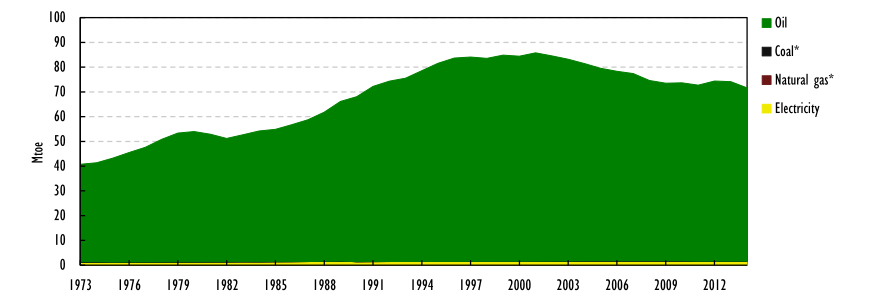
\includegraphics[width=\textwidth]{Transporte}
		\caption{Transporte.png}
		\label{fig:Transporte}
	\end{subfigure}
	%~ %add desired spacing between images, e. g. ~, \quad, \qquad, \hfill etc. 
	%(or a blank line to force the subfigure onto a new line)
	\begin{subfigure}[b]{1\textwidth}
		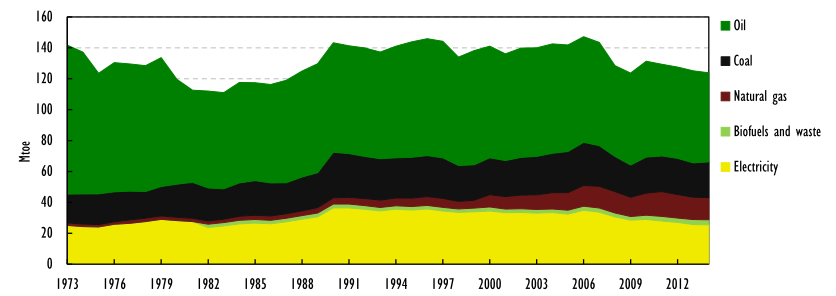
\includegraphics[width=\textwidth]{Industria}
		\caption{Industria.png}
		\label{fig:Industria}
	\end{subfigure}
	%~ %add desired spacing between images, e. g. ~, \quad, \qquad, \hfill etc. 
	%(or a blank line to force the subfigure onto a new line)
	\begin{subfigure}[b]{1\textwidth}
		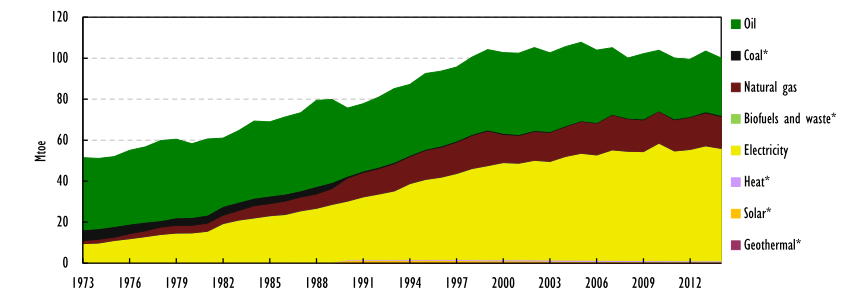
\includegraphics[width=\textwidth]{ResidencialComercial.png}
		\caption{Residencial y Transporte}
		\label{fig:Residencial}
	\end{subfigure}
	\caption{Consumo total de energía por sector y por fuente}\label{fig:sectores}
\end{figure}

En la figura \ref{fig:sectores} podemos apreciar el consumo de los energéticos por cada sector.\\

En el apartado \ref{fig:Transporte} podemos apreciar que el petróleo es la principal fuente de energía en el transporte y representa casi el 98 $\%$ del consumo energético del sector. La electricidad representa el 2.1$\%$ y el gas natural el 0.1 $\%$. Los biocombustibles no se consumen en el sector del transporte japonés.\\

En el apartado \ref{fig:Industria} se nota que la industria depende del petróleo en un 46,5 $\%$ de su demanda energética, mientras que el resto lo constituyen la electricidad (20.5 $\%$), el carbón (18.7 $\%$), el gas natural (11.6 $\%$) y los biocarburantes y residuos (2.7 $\%$). En la última década, la demanda de la industria se ha alejado del petróleo y la electricidad y ha pasado a un mayor uso de gas. La participación del petróleo y la electricidad en TFC cayó del 49.7 $\%$ y el 23.4 $\%$ en 2004, respectivamente, mientras que la participación del gas aumentó del 7.4 $\%$.\\


Por último en podemos ver en \ref {fig:Residencial} Los sectores residencial y comercial en su conjunto consumen principalmente electricidad (54.8 $\%$ de la demanda sectorial total en 2014), seguido por el petróleo (27.9 $\%$) y el gas (15.6 $\%$). Otras fuentes representaron el 1.7 $\%$ de la demanda. En la última década, la demanda ha pasado del uso del petróleo a más electricidad y gas. En 2004, la electricidad representó el 47.9 $\%$ de TFC y el gas natural el 13.8 $\%$, mientras que el petróleo tuvo una participación del 36.6 $\%$.\\
%\citep{InternationalEnergyAgency2016}\footnote{International Energy Agency 2016 p. 43}\\


\subsection{Vehículos Eléctricos}

En el sector del transporte, el aumento del número de vehículos eléctricos (VE) está determinado como una de las medidas para conseguir una sociedad baja en carbono, por lo que se prevé que la demanda de baterías recargables siga aumentando. El CRIEPI continúa la investigación y desarrollo de una batería de estado sólido que se puede utilizar como almacenamiento estacionario y también para vehículos eléctricos. También estamos desarrollando una tecnología de evaluación para lograr baterías de iones de litio de larga duración.\citep{Ryanair 2018}\footnote{Ryanair 2018 p. 59}\\

\section{Intensidad Energética}

La intensidad energética, medida como la relación entre el suministro total de energía primaria (TPES) por unidad de producto interior bruto real ajustado en función de la paridad del poder adquisitivo (PIB PPA), fue de 0,08 toneladas equivalentes de petróleo por USD 1 000 PPA (tep/USD 1 000) en 2015. La relación es inferior a los promedios de la AIE de 0,11 tep/USD 1 000 PPP.\\

 La intensidad energética de Japón es la decimoquinta más alta entre los países miembros de la AIE, es decir, alrededor de un nivel medio. La intensidad energética de Japón en 2015 fue un 19,7 $\%$ inferior a la de diez años antes, mientras que la intensidad media de la AIE disminuyó un 15,4 $\%$ durante el mismo período.\\ 
%(Figura 4.2).
Otro indicador común para las comparaciones internacionales es el consumo de energía per cápita.\\
%(véase la figura 4.3). 
La tasa de Japón de 3.4 tep per cápita al año es la decimotercera más baja entre los países miembros de la AIE, alrededor de un nivel medio.\citep{InternationalEnergyAgency2016}\footnote{International Energy Agency 2016 p. 43}\\



\bibliographystyle{apa}
\bibliography{Referencias.bib}

\end{document}
